\documentclass{article}
\usepackage[utf8]{inputenc}
\usepackage[polish]{babel}
\usepackage{graphicx}
\usepackage[T1]{fontenc}
\usepackage{wrapfig}
\usepackage{fancyhdr}
\usepackage{tabularx}
\usepackage{hyperref}
\usepackage{array}
\usepackage{multirow}




%\usepackage[a4paper,top=2cm,bottom=2cm,left=3cm,right=3cm,marginparwidth=1.75cm]{geometry}
\usepackage[includeheadfoot,
            left=1in,
            right=1in,
            top=1cm,
            bottom=1cm,
            headheight=1cm]{geometry}


\pagestyle{fancy}
\fancyhf{}
\renewcommand{\headrulewidth}{0pt}
\renewcommand{\footrulewidth}{0pt}

\fancypagestyle{firstpage}
{
    \fancyhead[L]       % <-----------------LEWA STRONA-----------------
        {

            \vspace{0.25cm}
            \textbf{\textit{Miłosz Grześkowiak}} \\
            {\textit{Rok 1 Informatyka Stosowana i Systemy Pomiarowe}} \\
            {\textit{17 Marca 2025}} \\
        }


    \fancyhead[R]   % <---------------------PRAWA STRONA------------
        {

             \vspace{0.25cm}
             \textit{18 Marca 2025}  \\
             {Prowadząca: } \\
             {\textit{dr Sylwia Owczarek}} \\

        }
}
\begin{document}
\textbf{ }\\
\textbf{ }\\
\thispagestyle{firstpage}
\centering
\section*{Ćwiczenie nr. 8}
\subsection*{Temat: Badanie rzutu poziomego; Badanie zderzeń sprężystych}
\textbf{ }\\
\textbf{ }\\
\textbf{ }\\
\textbf{ }\\
\begin{tabularx}{0.8\textwidth} {
  | >{\centering\arraybackslash}X |     % 1  }
  | >{\centering\arraybackslash}X |     % 2  }   LICZBA
  | >{\centering\arraybackslash}X |}    % 3  }   KOLUMN}
 \hline


 %---------------------------OPIS-------------------------------
 \#
 & 1. średnica kuli [mm]
 & 2. masa kuli [g]  \\
%---------------------------OPIS-------------------------------


\hline
\hline
%---------------------------DANE-------------------------------
\hline 1 & 19.47 & 32.5 \\
\hline 2 & 19.47 & 32.5 \\
\hline 3 & 19.46 & 32.5 \\
\hline 4 & 19.46 & 32.5 \\
\hline 5 & 19.46 & 32.5 \\
%---------------------------DANE-------------------------------
\hline
\end{tabularx}

\textbf{ }\\
\textbf{ }\\
\textbf{ }\\


\raggedright
    {
        {Dokładność wartości pomiaru średnicy} \\
        {$\Delta_1 = \pm0.01mm$ }\\
        \textbf{ }\\
        {Dokładność wartości pomiaru masy} \\
        {$\Delta_2 = \pm0.1g$ }\\
        \textbf{ }\\
    }
\centering
\subsection*{Zasięg kulki o $h_{stozek} = 18cm$}
\begin{tabularx}{0.8\textwidth} {
  | >{\centering\arraybackslash}X |     % 1  }
  | >{\centering\arraybackslash}X |
  | >{\centering\arraybackslash}X |
  | >{\centering\arraybackslash}X |}    % 3  }   KOLUMN}
 \hline

 %---------------------------OPIS-------------------------------
 \#
 & 1. zasięg wyrzucanej kuli o $h = 34cm$ [cm]
 & 2. zasięg wyrzucanej kuli o $h = 35cm$ [cm]
 & 3. zasięg wyrzucanej kuli o $h = 36cm$ [cm]\\
%---------------------------OPIS-------------------------------


\hline
\hline
%---------------------------DANE-------------------------------
\hline 1 & 28.7 & 29.5 & 30.0 \\
\hline 2 & 28.7 & 29.7 & 31.1 \\
\hline 3 & 29.4 & 30.5 & 31.3 \\
\hline 4 & 30.6 & 30.9 & 33.4 \\
%---------------------------DANE-------------------------------
\hline
\end{tabularx}

\textbf{} \\
\textbf{} \\

\raggedright
    {
        {Dokładność wartości pomiaru zasięgu} \\
        {$\Delta_1 = \pm0.1cm$ }\\
        \textbf{ }\\
    }

\centering
\subsection*{Zasięg kulki o $h_{stozek} = 20cm$}
\begin{tabularx}{0.8\textwidth} {
  | >{\centering\arraybackslash}X |     % 1  }
  | >{\centering\arraybackslash}X |
  | >{\centering\arraybackslash}X |
  | >{\centering\arraybackslash}X |}    % 3  }   KOLUMN}
 \hline

 %---------------------------OPIS-------------------------------
 \#
 & 1. zasięg wyrzucanej kuli o $h = 34cm$ [cm]
 & 2. zasięg wyrzucanej kuli o $h = 35cm$ [cm]
 & 3. zasięg wyrzucanej kuli o $h = 36cm$ [cm]\\
%---------------------------OPIS-------------------------------


\hline
\hline
%---------------------------DANE-------------------------------
\hline 1 & 27.9 & 28.9 & 30.0 \\
\hline 2 & 27.9 & 29.0 & 30.1 \\
\hline 3 & 28.2 & 29.1 & 31.0 \\
\hline 4 & 28.9 & 29.2 & 32.9 \\
%---------------------------DANE-------------------------------
\hline
\end{tabularx}

\textbf{} \\
\textbf{} \\

\raggedright
    {
        {Dokładność wartości pomiaru zasięgu} \\
        {$\Delta_1 = \pm0.1cm$ }\\
        \textbf{ }\\
    }


\centering

\section*{ZAGADNIENIA TEORETYCZNE}
\raggedright
{Eksperyment Badanie rzutu poziomego oraz Badanie zderzeń sprężystych ma na celu zbadanie zasad zachowania energii i pędu w układach fizycznych, w których występują zderzenia centralne oraz ruch ciała w polu grawitacyjnym. W tym eksperymencie wykorzystujemy dwie kulki o identycznych masach i średnicach, które są zawieszone na wahadle oraz na aparaturze pomiarowej.

1. Rzut poziomy

Rzut poziomy to ruch ciała, które zostaje wyrzucone z pewnej wysokości h z prędkością początkową skierowaną poziomo. W ruchu tym można wyróżnić dwa niezależne ruchy:

    \textbf{Ruch poziomy} – jednostajny, z prędkością $v_0$.

    \textbf{Ruch pionowy} – jednostajnie przyspieszony, z przyspieszeniem g (przyspieszenie ziemskie).

Czas lotu t w rzucie poziomym zależy od wysokości h i jest określony wzorem:
\[ t=\sqrt{\frac{2h}{g}} \]

Zasięg rzutu d (odległość, na jaką przemieści się ciało w poziomie) można obliczyć ze wzoru:
\[ d=v_0*t=v_0⋅\sqrt{\frac{2h}{g}} \]


gdzie $v_0$ to prędkość początkowa w kierunku poziomym.

2. Zderzenia sprężyste

Zderzenie sprężyste to takie zderzenie, w którym zarówno pęd, jak i energia kinetyczna układu są zachowane. W przypadku zderzenia centralnego dwóch ciał o jednakowych masach mm, prędkości ciał po zderzeniu można opisać za pomocą zasad zachowania pędu i energii.

Przed zderzeniem:

    Kulka 1 (wyrzucana) ma prędkość $v_1$.

    Kulka 2 (zawieszona) jest nieruchoma ($v_2=0$).

Po zderzeniu:

    Kulka 1 zatrzymuje się ($v_1′=0$).

    Kulka 2 uzyskuje prędkość $v_2′=v_1$.

Zasada zachowania pędu:
\[m*v_1+m*0=m*0+m*v_2′\]

Zasada zachowania energii kinetycznej:
\[ \frac12mv_{1}^2+\frac12m*0^2=\frac12m*0^2+\frac12mv′_{2}^2 \]

3. Wahadło

Wahadło wykorzystane w eksperymencie pozwala na kontrolowane uwolnienie kulki z określonej wysokości h. Energia potencjalna kulki na wysokości h jest zamieniana na energię kinetyczną w momencie uderzenia w drugą kulkę. Energia potencjalna Ep jest dana wzorem:
\[E_p=m*g*h\]

gdzie m to masa kulki, g to przyspieszenie ziemskie, a h to wysokość.

4. Cel eksperymentu

Celem eksperymentu jest zbadanie, jak zmiana wysokości h wpływa na odległość, na jaką druga kulka zostanie przesunięta po zderzeniu. Wykorzystując zasady zachowania energii i pędu, można przewidzieć teoretycznie, jak zmienne te wpływają na wynik eksperymentu, a następnie zweryfikować te przewidywania doświadczalnie. \\

Eksperyment ten pozwala na praktyczne zrozumienie podstawowych zasad mechaniki klasycznej, takich jak zasady zachowania energii i pędu, oraz na zbadanie wpływu różnych parametrów fizycznych na wynik zderzenia sprężystego.\\
\textbf{} \\
    Halliday, D., Resnick, R., \& Walker, J. (2015). Fizyka dla szkół wyższych. Tom 1: Mechanika. Warszawa: Wydawnictwo Naukowe PWN.

    Leyko, J. (2006). Mechanika ogólna. Warszawa: Wydawnictwo Naukowe PWN.}

\centering

\section*{OPIS DOŚWIADCZENIA}

{Doświadczenie polega na zderzeniu sprężystym dwóch kulek. Jedna zawieszona jest na napiętej lince, oraz przytwierdzona do elektromagnesu. Druga zaś leży na specjalnym łożu. Po zwolnieniu elektromagnesu, kulka druga wyrzucana jest na daną odległość dzięki zderzeniu sprężystemu. Eksperyment jest powtarzany kilkukrotnie, a następnie jest zmieniana wysokość elektromagnesu lub łoża.}

\section*{OPRACOWANIE WYNIKÓW POMIARÓW}

{W eksperymencie mierzona była odległość wyrzutu kulki po zderzeniu sprężystym z drugą kulką w zależności od wysokości elektromagnesu, oraz wysokości stożka (łoża), na którym leży kulka wyrzucana. Zmierzona również została masa oraz średnica kulki. Wyniki pomiarów zostały zamieszczone w trzech tabelach jako wstęp do sprawozdania. \\
Z wyników pomiarów zostały policzone średnie, odchylenia standardowe i procentowe. \\
\textbf{Wszystkie pomiary zostały wykonane za pomocą skryptu w języku Python$^{[1]}$} \\
Odchylenie standardowe zostało policzone ze wzoru
\[u(d) = \sqrt{\frac{1}{n(n-1)}\sum^n_{i=1}(d_i-d_{sr})^2}\]
a odchylenie procentowe ze wzoru
\[\frac{\Delta d}{d}*100\%\]
gdzie $\Delta d$ - odchylenie pomiaru, a $d$ - średnia pomiaru. \\
\begin{tabular}{|c|c|c|c|c|c|c|}
\hline
\multirow{2}{*}{} & \multicolumn{3}{c|}{stożek 18cm} & \multicolumn{3}{c|}{stożek 20cm} \\ \cline{2-7}
h [cm] & 34 & 35 & 36 & 34 & 35 & 36 \\ \hline
średnia [cm] & 29,35 & 30,15 & 31,45 & 28,22 & 29,05 & 31 \\ \hline
odchylenie standardowe & 0,77 & 0,57 & 1,22 & 0,4 & 0,11 & 1,16 \\ \hline
błąd standardowy & 0,38 & 0,28 & 0,61 & 0,2 & 0,05 & 0,58 \\ \hline
odchylenie procentowe [\%] & 2,64 & 1,89 & 3,91 & 1,44 & 0,38 & 3,75 \\ \hline
\end{tabular} \\
\textbf{} \\
Wyniki w powyższej tabeli pokazują, że wraz z zwiększaniem się wysokości elektromagnesu, zwiększa się zasięg wyrzucanej kulki zgodnie ze wzorem
\[E_p=m*g*h\]
Jednak w przypadku zwiększania się wysokości stożka, zasięg wyrzutu zmniejsza się (w porównaniu do tych samych wysokości elektromagnesu przy innej wysokości stożka). \\
Wynikać to może z różnicy wysokości w wyżej podanym wzorze, co możemy określić jako
\[E_p = m*g*(h_{elektromagnes} - h_{stozek})\] \\
Wyniki te zostały zobrazowane na Wykresie 1 na ostatniej stronie sprawozdania (wykonanym w języku Python$^{[1]}$).}\\
\subsection*{Oczekiwane wartości}
{Wiedząc, że zjawisko zachodzi za pomocą zasady zachowania energii i zderzeń sprężystych, oraz znając zależność \\
$m*g*h = \frac{1}{2}*m*v_{1}^{2}$
oraz
$v'_{2} = v_{1}$ \\
gdzie $v'_{2}$ - prędkość kulki wyrzucanej po zderzeniu; $v_{1}$ - prędkość kulki na wahadle. \\
Możemy wyliczyć prędkość, z jaką kulka będzie się poruszała, czyli:
\[v_{1}=\sqrt{2*g*h}\]
Wiedząc, że czas lotu możemy określić przekształcając wzór na spadek swobodny
\[t=\sqrt{\frac{2*h}{g}}\]
Możemy wyliczyć odległość wyrzutu kulki wiedząc, że odległość ta jest iloczynem prędkości i czasu
\[d = v_1*t\]
A więc po uproszczeniu
\[d=2*h\]
Dzięki temu możemy określić wartości oczekiwane dla naszego eksperymentu \\
\begin{tabular}{|c|c|c|c|c|c|c|}
\hline
\multirow{2}{*}{} & \multicolumn{3}{c|}{stożek 18cm} & \multicolumn{3}{c|}{stożek 20cm} \\
\cline{2-7}
h [cm] & 34 & 35 & 36 & 34 & 35 & 36 \\ \hline
prędkość [cm/s] & 17.71 & 18.28 & 18.79 & 16.57 & 17.15 & 17.71 \\ \hline
czas lotu [s] & 1.80 & 1.86 & 1.91 & 1.68 & 1.74 & 1.80 \\ \hline
odległość [cm] & 31.87 & 34.00 & 35.88 & 27.83 & 29.84 & 31.87 \\ \hline
\end{tabular} \\
}


\section*{WNIOSKI}

{Wyniki doświadczenia wskazują na to, że
\begin{itemize}
    \item Wraz ze wzrostem wysokości elektromagnesu, zasięg wyrzutu wzrasta
    \item Wraz ze wzrostem wysokości stożka, zasięg wyrzutu maleje
\end{itemize}
Jest to związane z Energią potencjalną, co zostało opisane w rozdziale "Opracowanie Wyników Pomiarów" \\
Zauważalnym swojego rodzaju błędem jest fakt, że różnica odległości wyliczonej od odległości zmierzonej jest odchylona o średnio $\pm2.14cm$. \\
Różnica ta może wynikać z wielu czynników takich jak:
\begin{enumerate}
    \item Opór powietrza
    \item Brak idealnej sprężystości zderzenia
    \item Błędy pomiarowe
\end{enumerate}
Sugerując się wartościami odchylenia standardowego i odchylenia procentowego, można wykluczyć błąd pomiarowy, gdyż nie są one na tyle duże, aby dorównać średniej odchylenia między odległościami wyliczonymi, a odległościami zmierzonymi. \\

Mimo błędów można zgodzić się z tezą, że zasięg wystrzału kulki wyrzucanej jest wprost proporcjonalny do różnicy wysokości między kulką na wahadle, a kulką wyrzucaną. \\
W celu zwiększenia dokładności pomiarów, należy określić w przyszłym eksperymencie opór powietrza, oraz wykonać eksperyment dla kulek o różnej masie (m) i średnicy ($\phi$).
}

\subsection*{Przypisy}
{[1] - \href{https://github.com/milosz0542/I-Pracownia-Fizyczna}{https://github.com/milosz0542/I-Pracownia-Fizyczna}}

\pagebreak
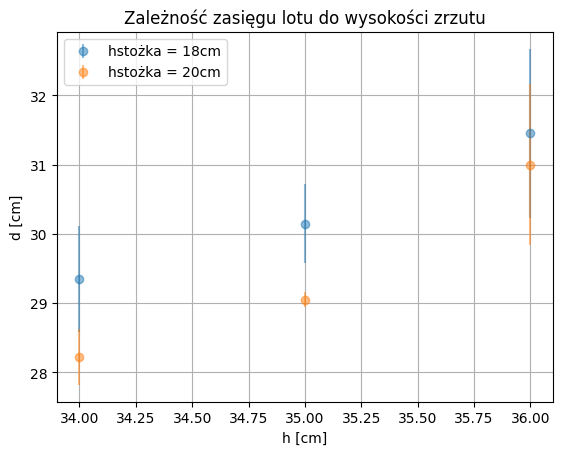
\includegraphics[angle=90, width=\textwidth, height=\textheight, keepaspectratio]{images/sprawozdanie1_1.png}
\footnotesize Wykres 1
\end{document}


%Dodatkowe uwagi:

1. Sprawozdanie może być pisane ręcznie. Proszę jednak o czytelność pisma!!!

2. Sprawozdanie MUSI zawierać wszystkie części (tabela pomiarową, teoria,
przebieg ćwiczenia, obliczenia, niepewności, wnioski i wykresy). Brak
jakiejkolwiek części kwalifikuje do zwrotu złożonego sprawozdania bez dalszego
sprawdzania.

3. Wykresy należy zamieszczać na osobnych kartkach (format A4). Wykonywać za
pomocą komputera lub ręcznie na papierze milimetrowym. Należy tak dobrać
skalę, aby wykres zajmował całą stronę.

4. Punktów pomiarowych naniesionych na wykresach nie łączymy! W przypadku
dopasowania prostej regresji, wraz punktami na wykresie należy nanieść prostą
regresji.

5. Na wykresach razem z punktami należy nanieść niepewności pomiarowe w formie
tzw. krzyży niepewności pomiarowych.

6. Do sprawozdania należy dołączyć kartkę pomiarową z ćwiczenia podpisaną przez
prowadzącego.

7. Przy zapisie wyników wraz z niepewnością obowiązuje zasada podawania 2 cyfr
znaczących (instrukcja ONP).

8. Niepewności pomiarowe w większości przypadków wyliczamy bazując na trzech
metodach:
a) gdy mamy pomiary skorelowane korzystamy z zależności 17 w instrukcji ONP,
b) gdy mamy pomiary nieskorelowane korzystamy z zależności 15 w ONP,
c) w przypadku dopasowywania prostych regresji, niepewności obliczamy ze
wzorów 6 i 7 w ONP.